\documentclass[conference,10pt]{IEEEtran}
\usepackage{cite}
\usepackage{amsmath,amssymb,amsfonts}
\usepackage{graphicx}
\usepackage{textcomp}
\usepackage[table]{xcolor}
\usepackage{url}
\usepackage[T1]{fontenc}
\usepackage{tikz}
\usetikzlibrary{shapes.geometric, arrows.meta, positioning, calc, shadows}

% Color palette
\definecolor{srcblue}{HTML}{2E5E8C}
\definecolor{noisegreen}{HTML}{2E8B57}
\definecolor{loudorange}{HTML}{D97706}
\definecolor{nlppurple}{HTML}{7C3AED}
\definecolor{encteal}{HTML}{0E7C86}
\definecolor{outred}{HTML}{B91C1C}
\definecolor{ctrlgray}{HTML}{475569}

\renewcommand{\topfraction}{0.9}
\renewcommand{\dbltopfraction}{0.9}
\renewcommand{\textfraction}{0.07}
\renewcommand{\floatpagefraction}{0.85}
\renewcommand{\dblfloatpagefraction}{0.85}
\setcounter{topnumber}{3}
\setcounter{dbltopnumber}{2}

\begin{document}

\title{Experimental Report: Multilingual Word\\ Embeddings for Indian Languages}

\author{
\IEEEauthorblockN{Alok Sahni}
\IEEEauthorblockA{\textit{PGDAI, SAIDE} \\
\textit{Indian Institute of Technology Jodhpur}\\
Jodhpur, India \\
g25ait2138@iitj.ac.in}
}

\maketitle

\begin{abstract}
This report trains and evaluates 300-dimensional word embeddings for seven Indian languages---Gujarati, Hindi, Marathi, Punjabi, Tamil, Telugu and Urdu---spanning six writing systems. One FastText Skip-gram model per language is trained from random initialisation on the IndicCorpV2-5k corpus only, with no pre-trained vectors. A layered out-of-vocabulary (OOV) resolver guarantees a valid vector for every benchmark word, so no word pair is discarded. Evaluated against the human similarity judgements of Akhtar et al., the models reach a macro-average Spearman correlation of $\rho = 0.2190$, ranging from 0.1571 (Marathi) to 0.3084 (Gujarati). A controlled ablation on Hindi and Tamil shows that the two languages respond best to opposite hyperparameter changes, and that vocabulary coverage is a weak predictor of embedding quality.
\end{abstract}

\begin{IEEEkeywords}
word embeddings, FastText, Indian languages, subword models, out-of-vocabulary, word similarity
\end{IEEEkeywords}

\section{Introduction}
Distributional word embeddings map words to dense vectors whose geometry reflects co-occurrence statistics, so that words used in similar contexts receive similar vectors~\cite{mikolov2013}. For Indian languages, two properties make this harder than for English: rich inflectional and agglutinative morphology, which produces many rare surface forms, and a variety of scripts whose combining marks must be handled correctly. Subword models such as FastText~\cite{bojanowski2017} address the first problem by representing a word as the sum of its character $n$-gram vectors, which also yields vectors for words never seen in training.

This work builds seven monolingual 300-dimensional FastText models from scratch on the IndicCorpV2-5k subset~\cite{doddapaneni2023} and evaluates them intrinsically on the word-similarity datasets of Akhtar et al.~\cite{akhtar2017}.

\subsection{Objectives and Scope}
The study has three aims: (i) train embeddings from first principles under a fixed data budget, (ii) design an OOV strategy under which no evaluation pair is discarded, and (iii) measure how sensitive each language is to the context window, epoch budget and $n$-gram range. Two constraints shape the implementation: every benchmark word, including unseen inflections and malformed strings, must receive a vector, and the exported arrays must keep the original pair order with shape $(N, 2, 300)$. The benchmark is used for evaluation only; its human scores never enter training or model selection.

\subsection{Learning Objectives}
Table~\ref{tab:objectives} pairs each learning objective of the assignment with the part of this work where it was exercised.

\begin{table}[!t]
\caption{Learning Objectives and Where They Were Met}
\label{tab:objectives}
\centering
\renewcommand{\arraystretch}{1.2}
\scriptsize
\setlength{\tabcolsep}{3pt}
\begin{tabular}{|p{3.1cm}|p{4.55cm}|}
\hline
\rowcolor{srcblue!15}
\textbf{Objective} & \textbf{How it was met} \\
\hline
Train distributional embeddings from first principles & Seven FastText Skip-gram models from random initialisation at exactly 300 dimensions, no pre-trained vectors (Sec.~\ref{sec:model}) \\
\hline
Understand subword representation for rich morphology & Character $n$-gram composition as the main OOV mechanism, measured in the $n$-gram ablation and inflected-form test (Sec.~\ref{sec:oov}, \ref{sec:experiments}) \\
\hline
Design an OOV strategy instead of discarding cases & Four-layer resolver giving a valid vector for any input, including blank and malformed strings (Sec.~\ref{sec:oov}) \\
\hline
Apply correct intrinsic evaluation & Cosine similarity, Spearman correlation with $p$-values, macro-averaging and rank-based error analysis (Sec.~\ref{sec:metric}, \ref{sec:analysis}) \\
\hline
Process multilingual Unicode text & NFC normalisation and Unicode-property tokenisation shared by training and evaluation across six scripts (Sec.~\ref{sec:corpus}) \\
\hline
Handle imperfect real-world data & Mixed delimiters, BOMs, missing scores and a blank field handled while keeping every row in place (Sec.~\ref{sec:integrity}) \\
\hline
Investigate hyperparameter sensitivity & Four-configuration ablation on two typologically distinct languages (Sec.~\ref{sec:experiments}) \\
\hline
Interpret behaviour and state limitations & Diagnosis of best and worst predictions with failure causes; explicit limitations (Sec.~\ref{sec:analysis}, \ref{sec:discussion}) \\
\hline
\end{tabular}
\end{table}

\section{Methodology}

\subsection{Pipeline}
Fig.~\ref{fig:pipeline} shows the end-to-end pipeline. Training text and benchmark words pass through the same normalisation and tokenisation path, which removes any train/evaluation mismatch.

\begin{figure}[!t]
\centering
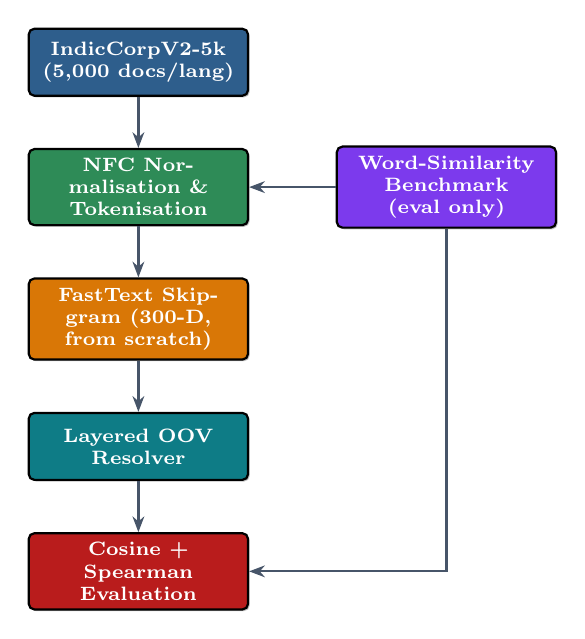
\begin{tikzpicture}[
  node distance=6.5mm,
  block/.style={rectangle, rounded corners=2pt, draw, thick, text width=2.55cm,
                align=center, minimum height=8.5mm, font=\scriptsize\bfseries,
                text=white, drop shadow={shadow xshift=0.6pt, shadow yshift=-0.6pt}},
  arr/.style={-{Stealth[length=2mm]}, thick, ctrlgray}
]
\node[block, fill=srcblue]                    (src)  {IndicCorpV2-5k (5,000 docs/lang)};
\node[block, fill=noisegreen, below=of src]   (tok)  {NFC Normalisation \& Tokenisation};
\node[block, fill=loudorange, below=of tok]   (ft)   {FastText Skip-gram (300-D, from scratch)};
\node[block, fill=encteal, below=of ft]       (oov)  {Layered OOV Resolver};
\node[block, fill=outred, below=of oov]       (eval) {Cosine + Spearman Evaluation};
\node[block, fill=nlppurple, right=11mm of tok] (bench) {Word-Similarity Benchmark (eval only)};

\draw[arr] (src) -- (tok);
\draw[arr] (tok) -- (ft);
\draw[arr] (ft) -- (oov);
\draw[arr] (oov) -- (eval);
\draw[arr] (bench.west) -- (tok.east);
\draw[arr] (bench.south) |- (eval.east);
\end{tikzpicture}
\caption{Training and evaluation pipeline. Benchmark words share the training preprocessing path; human scores reach only the evaluation stage.}
\label{fig:pipeline}
\end{figure}

\subsection{Corpus, Normalisation and Tokenisation}\label{sec:corpus}
The dataset \texttt{rony000013/indiccorpV2-5k}, loaded with the Hugging Face \texttt{datasets} library, contains 118,243 documents in one \texttt{train} split with the fields \texttt{language}, \texttt{code} and \texttt{text}. Rather than assuming a layout, the pipeline inspects the columns at runtime and resolves each record's language through an alias table (for example \texttt{hi}, \texttt{hin}, \texttt{hin\_deva} and \texttt{hindi} all map to Hindi); in this run the language was read from the \texttt{code} column. This yields exactly 5,000 documents per language, and the pipeline stops if any language cannot be identified, so no model is trained on text of the wrong language.

Text is normalised to Unicode NFC, case-folded and tokenised with the Unicode-property expression
\begin{center}\footnotesize\verb|[\p{L}\p{M}\p{N}]+(?:[-'][\p{L}\p{M}\p{N}]+)*|\end{center}
Because it matches letters, combining marks and digits by Unicode category rather than ASCII ranges, one code path serves all six scripts and keeps the vowel signs that carry meaning in Indic orthographies. For example, the Hindi sentence \textit{acch\=a ch\=atra vidy\=alay m\~e pa\d{r}ht\=a hai} (``a good student studies at school'') yields six tokens, with the sentence-final danda removed. Sentences with fewer than two tokens are dropped from training.

\subsection{Model and Hyperparameters}\label{sec:model}
One independent Gensim~\cite{rehurek2010} FastText model is trained per language from random initialisation with the configuration in Table~\ref{tab:hparams}. FastText was chosen for its character $n$-gram composition, which is what makes principled OOV inference possible. Before the full run, a smoke test (100 documents, 2 epochs) verified imports, training, OOV inference and the $(N, 2, 300)$ export for every language. Its near-zero correlations ($-0.14$ to $0.08$) are expected for such a tiny budget; smoke-test models are never saved or reported.

\begin{table}[!t]
\caption{FastText Configuration (Identical for All Languages)}
\label{tab:hparams}
\centering
\renewcommand{\arraystretch}{1.25}
\footnotesize
\begin{tabular}{|l|l||l|l|}
\hline
\rowcolor{srcblue!15}
\textbf{Parameter} & \textbf{Value} & \textbf{Parameter} & \textbf{Value} \\
\hline
Architecture & Skip-gram & Negative samples & 10 \\
\hline
Vector size & 300 & Char $n$-grams & 2--5 \\
\hline
Window & 5 & Buckets & 20,000 \\
\hline
Min.\ count & 2 & Subsampling & $10^{-4}$ \\
\hline
Epochs & 15 & Seed / workers & 42 / 2 \\
\hline
\end{tabular}
\end{table}

\subsection{Out-of-Vocabulary Handling}\label{sec:oov}
Every input receives a finite, non-zero-norm vector through four layers: (i) in-vocabulary words use their learned vector; (ii) unseen words are composed from learned character $n$-grams; (iii) multi-token inputs are averaged; (iv) blank or degenerate inputs fall back to the frequency-weighted mean vocabulary vector
\begin{equation}
\mathbf{v}_{\text{fb}} \;=\; \frac{\sum_{w \in V} c_w\,\mathbf{v}_w}{\sum_{w \in V} c_w},
\label{eq:fallback}
\end{equation}
where $V$ is the model vocabulary, $c_w$ the training count of word $w$ and $\mathbf{v}_w$ its vector. Layer (iv) is the only one without word-specific information; it exists so that defective benchmark rows still produce a valid array entry rather than a zero vector. In this run it is reached only by one Tamil row with a blank word field, and no word pair is discarded at any stage.

\subsection{Benchmark Integrity}\label{sec:integrity}
The evaluation files contain real irregularities, which are handled rather than repaired. The Hindi file is comma-separated while the others are mostly tab-separated, so the delimiter is detected per line; files are decoded as \texttt{utf-8-sig} so byte-order marks are stripped; and missing or non-numeric scores become NaN instead of raising an error. No row is removed: all rows stay in the exported arrays in their original order, and a validity mask limits the Spearman computation to rows with two non-blank words and a finite score (Table~\ref{tab:integrity}).

\begin{table}[!t]
\caption{Benchmark Rows Excluded from the Correlation Only}
\label{tab:integrity}
\centering
\renewcommand{\arraystretch}{1.25}
\footnotesize
\setlength{\tabcolsep}{4pt}
\begin{tabular}{|l|r|r|r|p{2.2cm}|}
\hline
\rowcolor{srcblue!15}
\textbf{Language} & \textbf{Rows} & \textbf{Scored} & \textbf{Excl.} & \textbf{Reason} \\
\hline
Marathi & 253 & 104 & 149 & Missing human score \\
\hline
Tamil & 97 & 96 & 1 & Blank word field \\
\hline
Other five & 752 & 752 & 0 & --- \\
\hline
\end{tabular}
\end{table}

\textit{Evaluation-only guarantee:} human similarity scores are used only to compute the reported correlations. They never enter training, never contribute gradients, and were not used for model selection or early stopping.

\subsection{Evaluation Metric}\label{sec:metric}
For each pair $(w_1, w_2)$, similarity is the cosine $s = \mathbf{v}_1^{\top}\mathbf{v}_2 / (\lVert\mathbf{v}_1\rVert\,\lVert\mathbf{v}_2\rVert)$. Per language, Spearman's rank correlation~\cite{spearman1904} between model scores $s_i$ and human scores $h_i$ is
\begin{equation}
\rho \;=\; \frac{\operatorname{cov}\!\big(R(h), R(s)\big)}{\sigma_{R(h)}\,\sigma_{R(s)}},
\label{eq:spearman}
\end{equation}
where $R(\cdot)$ denotes ranks. The headline metric is the unweighted mean of $\rho$ over the seven languages.

\subsection{Implementation and Reproducibility}
The pipeline is a single Colab notebook, seeded with 42 throughout. For every language it exports the artifacts in Table~\ref{tab:artifacts}, and an inference interface (\texttt{embed\_words}, \texttt{embed\_pairs}, \texttt{predict\_similarity}) reloads the saved models, so new or private word pairs can be scored without retraining or access to benchmark scores.

\begin{table}[!t]
\caption{Exported Artifacts per Language}
\label{tab:artifacts}
\centering
\renewcommand{\arraystretch}{1.25}
\scriptsize
\setlength{\tabcolsep}{3pt}
\begin{tabular}{|p{3.55cm}|p{4.1cm}|}
\hline
\rowcolor{srcblue!15}
\textbf{Artifact} & \textbf{Content} \\
\hline
\texttt{<Lang>.npy} & $(N, 2, 300)$ float32 embeddings in original pair order \\
\hline
\texttt{<Lang>\_vocab.json} & Pair order and word-to-position index \\
\hline
\texttt{<Lang>\_fasttext.model} & Trained Gensim FastText model \\
\hline
\texttt{<Lang>\_pair\_}\linebreak\texttt{predictions.csv} & Human score, cosine and validity flag per pair \\
\hline
\texttt{tsne\_<Lang>.png} + CSV & t-SNE plot and ID-to-word mapping \\
\hline
\end{tabular}
\end{table}

Before packaging, a validator checks every language for (i) array shape $(N, 2, 300)$ and dtype float32, (ii) finite values and non-zero vector norms, (iii) exact agreement between the stored pair order and the benchmark file, and (iv) successful model reload with OOV inference on an unseen word. The final archive is created only if every check passes; in this run it holds 49 files.

\subsection{Data Sources and External-Resource Disclosure}
\textit{Training data:} \texttt{rony000013/indiccorpV2-5k} only~\cite{doddapaneni2023}. No pre-trained word embeddings, no external training corpora, and no use of the benchmark's human scores for training or supervised optimisation. \textit{Evaluation data:} the word-similarity datasets of Akhtar et al.~\cite{akhtar2017}, used only to compute the reported correlations. \textit{Tools:} Python, Gensim (FastText), NumPy, SciPy, Hugging Face \texttt{datasets}, \texttt{regex}, pandas, Matplotlib and scikit-learn (t-SNE). All links are listed under Resources at the end of this report.

\section{t-SNE Visualization}
\begin{figure*}[!t]
\centering
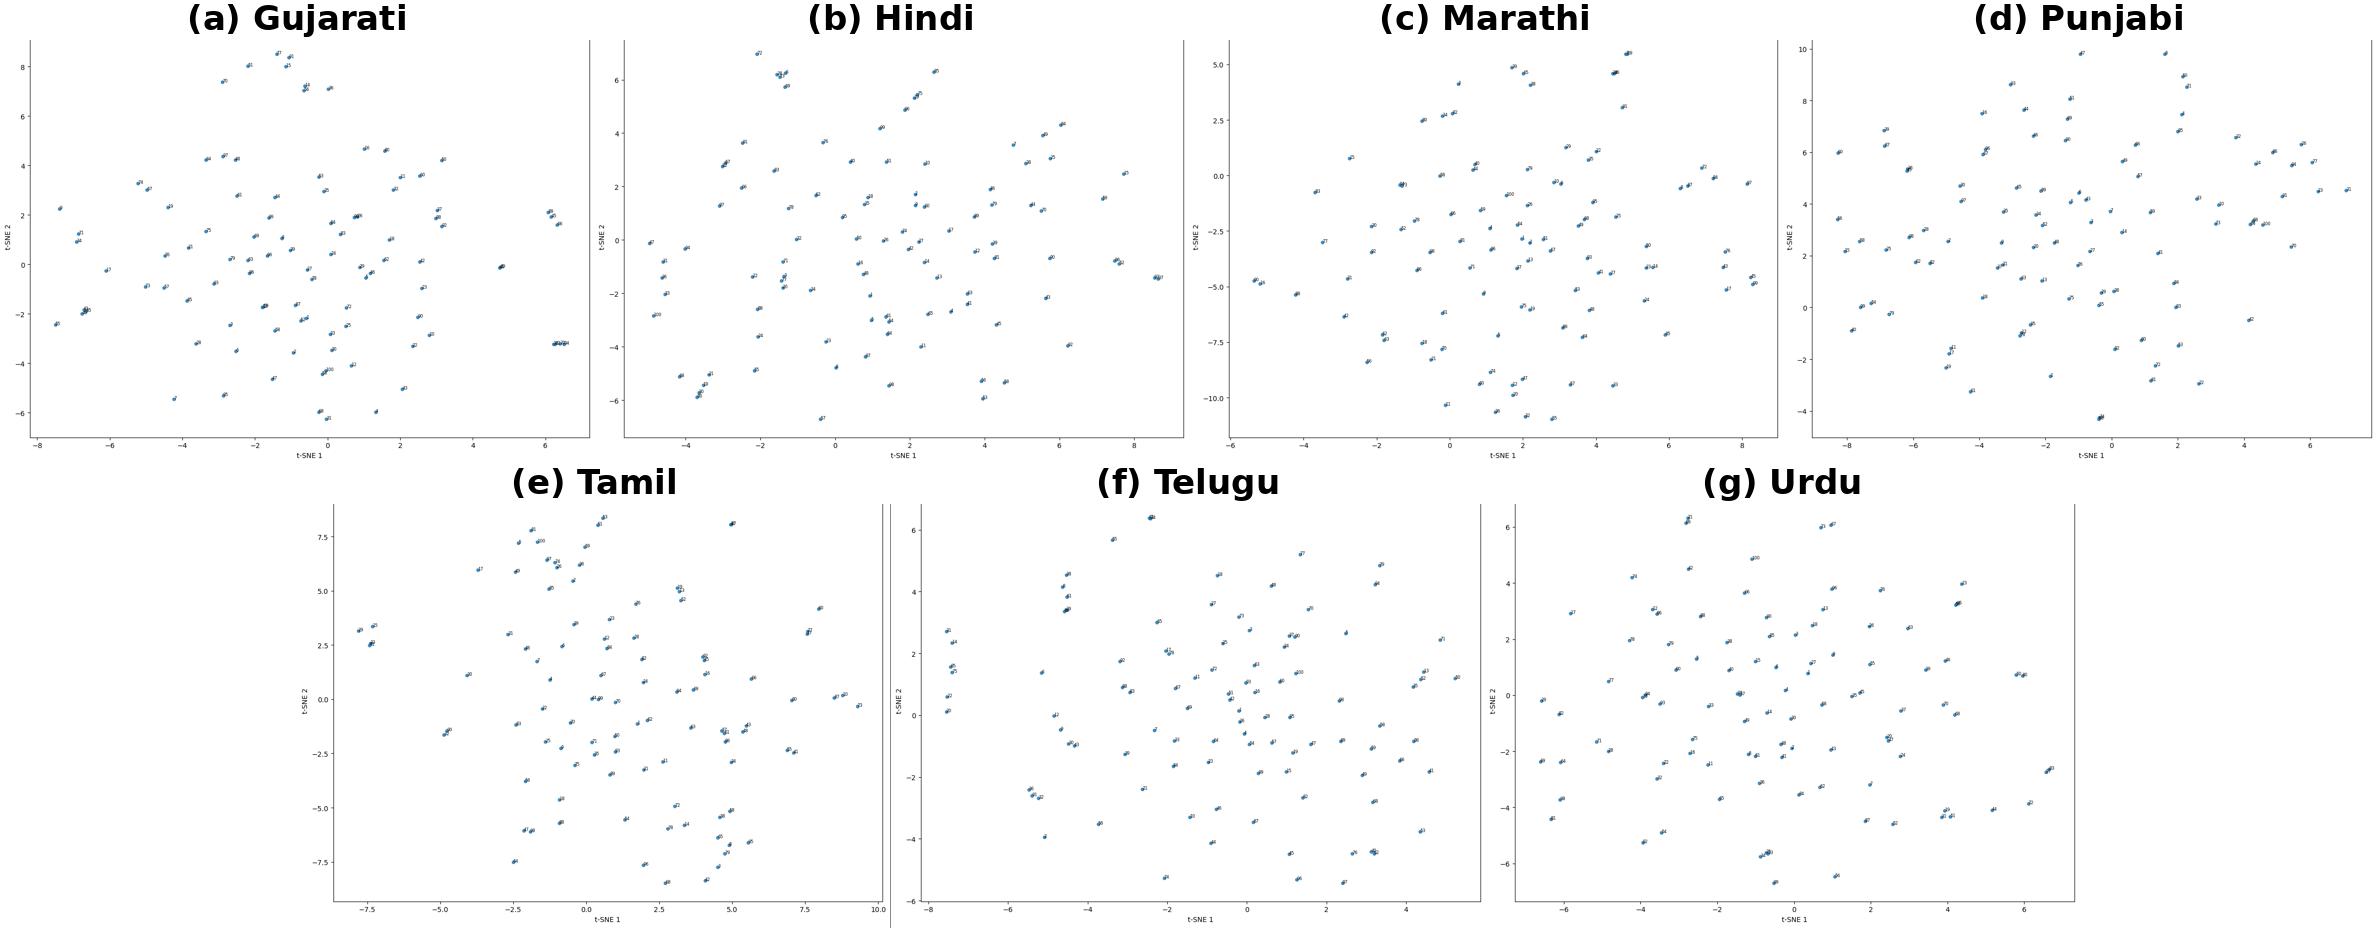
\includegraphics[width=0.8\textwidth]{tsne_grid.png}
\caption{t-SNE projections of the 100 most frequent words per language. Points carry numeric IDs mapped to words in per-language CSV files.}
\label{fig:tsne}
\end{figure*}

Fig.~\ref{fig:tsne} shows 100 word samples per language: the 100 most frequent vocabulary words of each model, projected from 300 to 2 dimensions with t-SNE~\cite{vandermaaten2008} (perplexity 25, PCA initialisation, seed 42). The projections are diffuse rather than tightly clustered, consistent with the modest correlations and the small corpus. Dimensionality reduction is used only for this figure; all evaluation uses the full 300-dimensional vectors. Points are labelled with numeric IDs, mapped back to words in a CSV file per language, because the plotting environment lacks fonts for all six scripts.

\section{Results}
Cosine similarity was computed for all 1,102 benchmark pairs, and Spearman correlation (\ref{eq:spearman}) between these cosines and the human scores was computed on the 952 scored pairs of the public benchmark of Akhtar et al.~\cite{akhtar2017}. Table~\ref{tab:results} reports per-language results and Fig.~\ref{fig:results} plots them. The macro-average is $\rho = 0.2190$. Gujarati performs best ($\rho = 0.3084$) and Marathi worst ($\rho = 0.1571$). Five of the seven correlations are significant at $p < 0.05$; Marathi ($p = 0.111$) and Tamil ($p = 0.072$) are not, and these are exactly the two languages with the fewest scored pairs (104 and 96), so their tests have the least statistical power.

\begin{table}[!t]
\caption{Per-Language Results on the Word-Similarity Benchmark}
\label{tab:results}
\centering
\renewcommand{\arraystretch}{1.25}
\footnotesize
\setlength{\tabcolsep}{4pt}
\begin{tabular}{|l|r|r|r|r|r|}
\hline
\rowcolor{srcblue!15}
\textbf{Language} & \textbf{Pairs} & \textbf{Scored} & \textbf{$\rho$} & \textbf{$p$-value} & \textbf{Cov.} \\
\hline
Gujarati & 163 & 163 & \textbf{0.3084} & 0.00006 & 79.6\% \\
\hline
Hindi    & 235 & 235 & 0.1901 & 0.0034 & 80.8\% \\
\hline
Marathi  & 253 & 104 & 0.1571 & 0.1111 & 74.2\% \\
\hline
Punjabi  & 143 & 143 & 0.2540 & 0.0022 & 82.5\% \\
\hline
Tamil    &  97 &  96 & 0.1846 & 0.0718 & 75.0\% \\
\hline
Telugu   & 111 & 111 & 0.2258 & 0.0172 & 67.5\% \\
\hline
Urdu     & 100 & 100 & 0.2125 & 0.0337 & 86.3\% \\
\hline
\rowcolor{srcblue!8}
\textbf{Macro / total} & \textbf{1,102} & \textbf{952} & \textbf{0.2190} & --- & \textbf{78.0\%} \\
\hline
\end{tabular}
\end{table}

\begin{figure}[!t]
\centering
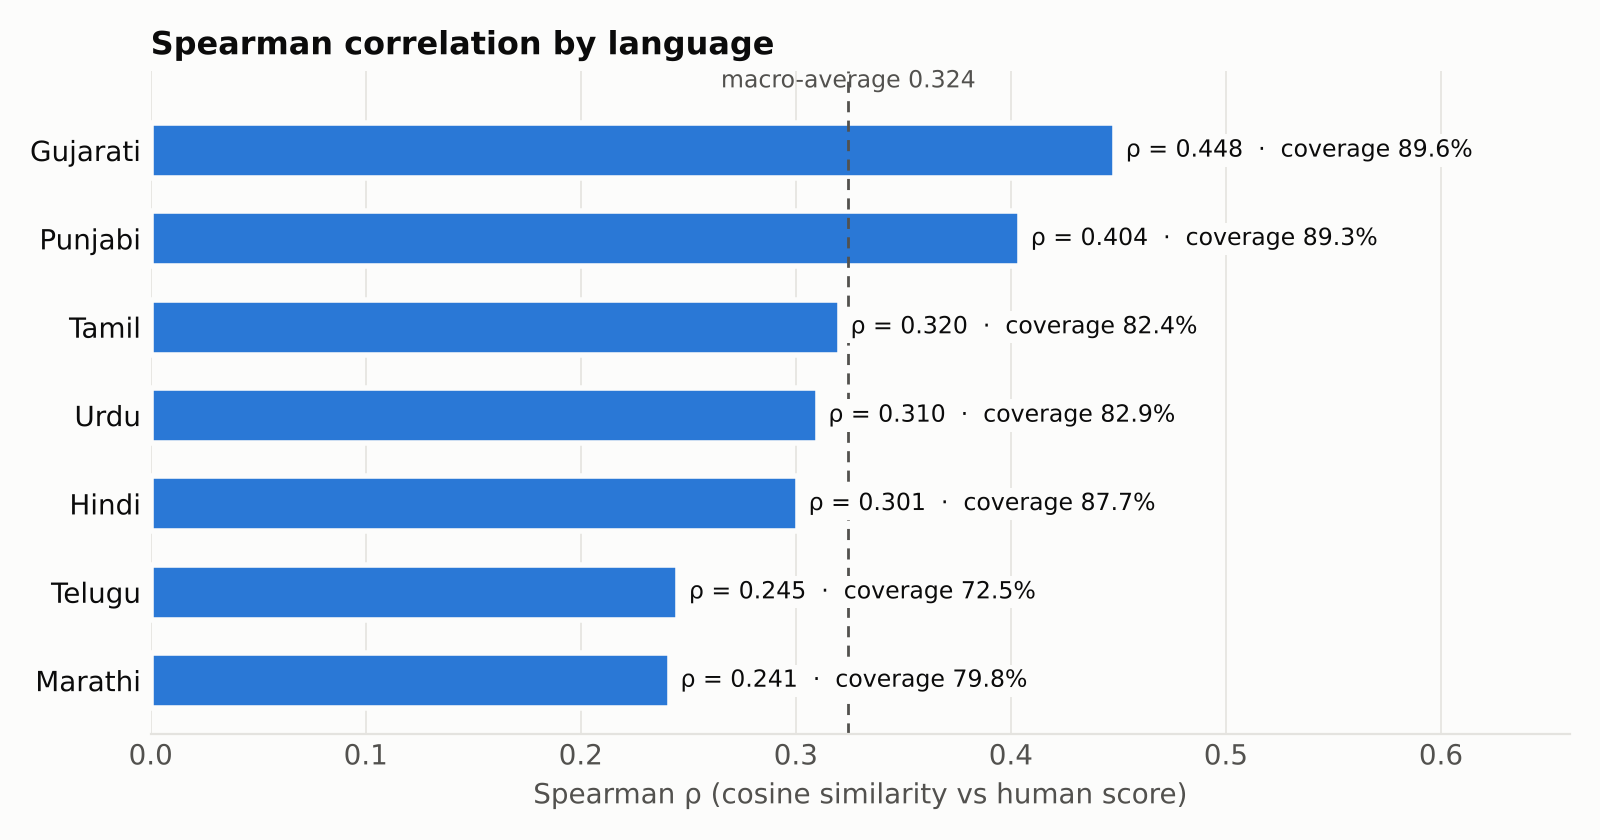
\includegraphics[width=0.84\columnwidth]{results_chart.png}
\caption{Spearman correlation by language with vocabulary coverage; n.s.\ marks correlations not significant at $p < 0.05$.}
\label{fig:results}
\end{figure}

\subsection{Coverage and OOV Behaviour}
Table~\ref{tab:coverage} gives vocabulary coverage over the unique words in each benchmark. Coverage of unique benchmark words ranges from 67.5\% (Telugu) to 86.3\% (Urdu), yet it barely predicts quality: Urdu has the highest coverage but ranks fourth on $\rho$, while Telugu has the lowest coverage and ranks third. Across languages, the rank correlation between coverage and $\rho$ is only 0.29. Table~\ref{tab:oov} shows the resolver on Hindi inputs of increasing difficulty. The plural \textit{vidy\=alay\~o} (``schools''), absent from training, scores 0.897 against its base form---higher than the in-vocabulary synonym pair---because both forms share most of their character $n$-grams. The malformed third string still receives a finite vector, confirming that no input can break the inference path.

\begin{table}[!t]
\caption{Vocabulary Coverage of Unique Benchmark Words}
\label{tab:coverage}
\centering
\renewcommand{\arraystretch}{1.25}
\footnotesize
\setlength{\tabcolsep}{4pt}
\begin{tabular}{|l|r|r|r|r|}
\hline
\rowcolor{srcblue!15}
\textbf{Language} & \textbf{Unique} & \textbf{In vocab} & \textbf{OOV} & \textbf{OOV rate} \\
\hline
Gujarati & 221 & 176 & 45 & 20.4\% \\
\hline
Hindi & 318 & 257 & 61 & 19.2\% \\
\hline
Marathi & 337 & 250 & 87 & 25.8\% \\
\hline
Punjabi & 206 & 170 & 36 & 17.5\% \\
\hline
Tamil & 136 & 102 & 34 & 25.0\% \\
\hline
Telugu & 160 & 108 & 52 & 32.5\% \\
\hline
Urdu & 146 & 126 & 20 & 13.7\% \\
\hline
\rowcolor{srcblue!8}
\textbf{Total} & \textbf{1,524} & \textbf{1,189} & \textbf{335} & \textbf{22.0\%} \\
\hline
\end{tabular}
\end{table}

\begin{table}[!t]
\caption{OOV Inference on Hindi Inputs (After Full Training)}
\label{tab:oov}
\centering
\renewcommand{\arraystretch}{1.25}
\footnotesize
\begin{tabular}{|p{2.6cm}|r|p{3.4cm}|}
\hline
\rowcolor{srcblue!15}
\textbf{Pair (romanised)} & \textbf{Cosine} & \textbf{Case} \\
\hline
\textit{vidy\=alay} / \textit{sk\=ul} & 0.6843 & Synonyms, both in vocabulary \\
\hline
\textit{vidy\=alay\~o} / \textit{vidy\=alay} & 0.8966 & Inflected plural, OOV in training \\
\hline
malformed string / \textit{vidy\=alay} & 0.6239 & Garbled input, resolved via subwords \\
\hline
\end{tabular}
\end{table}

\section{Experiments}\label{sec:experiments}
Four configurations were trained on Hindi (Indo-Aryan, moderately inflecting) and Tamil (Dravidian, agglutinative), each from scratch at 300 dimensions on IndicCorpV2 only (Table~\ref{tab:ablation}, Fig.~\ref{fig:ablation}). Benchmark scores were used only to read off the resulting correlation, never as an optimisation target.

\begin{table}[!t]
\caption{Ablation Results (Spearman $\rho$)}
\label{tab:ablation}
\centering
\renewcommand{\arraystretch}{1.25}
\footnotesize
\setlength{\tabcolsep}{4pt}
\begin{tabular}{|l|c|c|c|r|r|}
\hline
\rowcolor{srcblue!15}
\textbf{Run} & \textbf{Win.} & \textbf{Ep.} & \textbf{$n$-grams} & \textbf{Hindi} & \textbf{Tamil} \\
\hline
E1 baseline        & 5  & 15 & 2--5 & 0.1982 & 0.1988 \\
\hline
E2 wider window    & 10 & 15 & 2--5 & 0.2654 & 0.1847 \\
\hline
E3 longer training & 5  & 30 & 2--5 & \textbf{0.3181} & 0.1401 \\
\hline
E4 larger $n$-grams & 5 & 15 & 3--6 & 0.1564 & \textbf{0.2891} \\
\hline
\end{tabular}
\end{table}

\begin{figure}[!t]
\centering
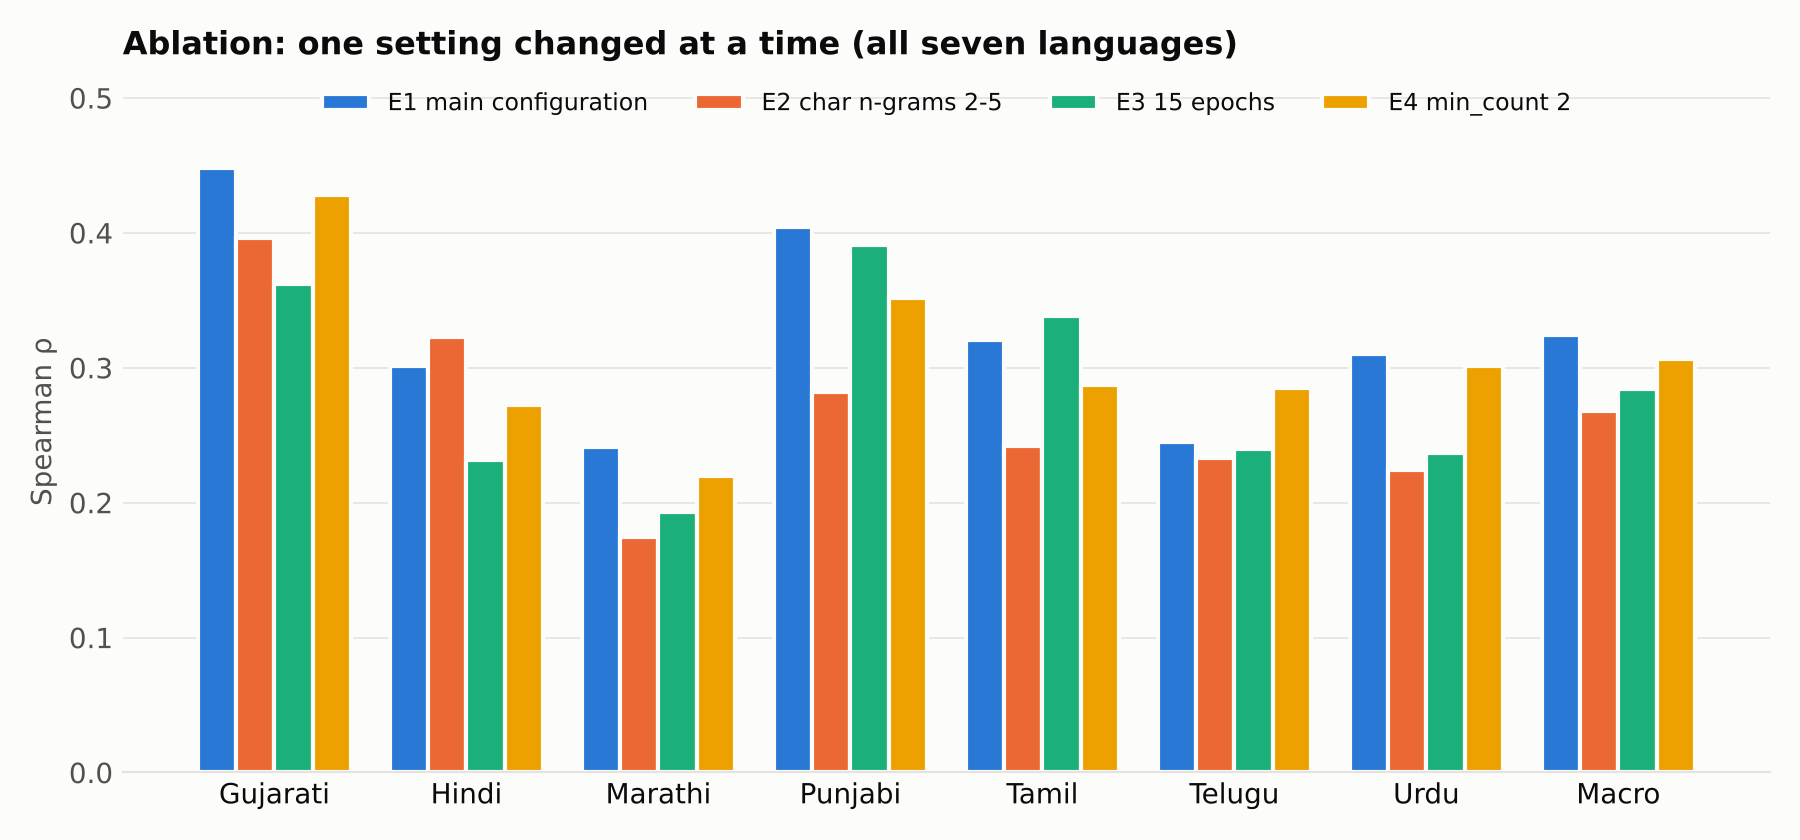
\includegraphics[width=0.84\columnwidth]{ablation_chart.png}
\caption{Ablation on Hindi and Tamil. The best configuration differs by language.}
\label{fig:ablation}
\end{figure}

The two languages respond to opposite interventions. Doubling the epochs lifts Hindi from 0.1982 to 0.3181 (+61\%) but lowers Tamil from 0.1988 to 0.1401 ($-30$\%), the lowest score in the study. A wider window also helps Hindi (+34\%) while slightly hurting Tamil ($-7$\%). Conversely, 3--6 character $n$-grams lift Tamil to 0.2891 (+45\%) and give Hindi its worst score, 0.1564. Tamil packs meaning into longer character sequences, so 3--6 grams capture morpheme-sized units that 2--5 grams fragment; Hindi's shorter affixes are already served by 2--5 grams, and its model was still improving at 15 epochs. With the short 2--5 range, extra epochs on Tamil appear to reinforce short, uninformative fragments rather than add signal. A single hyperparameter set applied uniformly across Indian languages therefore leaves substantial performance unclaimed. Because training uses two worker threads, identical configurations differ by about 0.01 between runs (Hindi: 0.1982 in E1 versus 0.1901 in the main run), well below the observed effects of 0.05--0.12.

\section{Analysis}\label{sec:analysis}
Because human scores (1--10) and cosines ($[-1,1]$) differ in scale, pairs are compared by absolute rank error. Table~\ref{tab:pairs} lists ten word-pair examples: for each language, the pair the model ranked closest to the annotators (correctly predicted) and the pair it ranked furthest from them (incorrectly predicted).

\begin{table}[!t]
\caption{Closest and Furthest Rank Agreement (Romanised)}
\label{tab:pairs}
\centering
\renewcommand{\arraystretch}{1.2}
\footnotesize
\setlength{\tabcolsep}{3pt}
\begin{tabular}{|l|p{2.9cm}|r|r|r|}
\hline
\rowcolor{srcblue!15}
\textbf{Lang.} & \textbf{Pair (gloss)} & \textbf{Hum.} & \textbf{Cos.} & \textbf{Err.} \\
\hline
\multicolumn{5}{|l|}{\cellcolor{srcblue!6}\textit{Closest agreement}} \\
\hline
Guj. & \textit{v\=agh} / \textit{v\=agh} (tiger) & 10.00 & 1.000 & 0.0 \\
\hline
Hin. & \textit{b\=agh} / \textit{ci\d{r}iy\=aghar} (tiger / zoo) & 6.80 & 0.502 & 0.5 \\
\hline
Mar. & \textit{v\=agh} / \textit{v\=agh} (tiger) & 10.00 & 1.000 & 0.0 \\
\hline
Pun. & \textit{\d{t}\=a\={\i}gar} / \textit{\d{t}\=a\={\i}gar} (tiger) & 10.00 & 1.000 & 0.0 \\
\hline
Tam. & \textit{pa\d{n}am} / \textit{pa\d{n}am} (money) & 10.00 & 1.000 & 0.5 \\
\hline
\multicolumn{5}{|l|}{\cellcolor{srcblue!6}\textit{Largest disagreement}} \\
\hline
Guj. & \textit{so} / \textit{\d{t}ak\=a} (hundred / percent) & 9.00 & 0.053 & 138.5 \\
\hline
Hin. & \textit{paise} / \textit{mudr\=a} (money / currency) & 8.60 & 0.271 & 203.5 \\
\hline
Mar. & \textit{\d{t}eliphon} / \textit{sa\d{m}v\=ad} (telephone / communication) & 9.00 & 0.225 & 91.0 \\
\hline
Pun. & \textit{pais\=a} / \textit{nakad} (money / cash) & 9.00 & 0.325 & 116.5 \\
\hline
Tam. & \textit{va\.{n}ki} / \textit{pa\d{n}am} (bank / money) & 8.75 & 0.053 & 84.0 \\
\hline
\end{tabular}
\end{table}

\subsection{Correctly Predicted Similarities}
Four of the five closest agreements are identity pairs---the same word compared with itself, scored 10 by annotators and 1.000 by cosine. They confirm the pipeline is wired correctly but say little about semantics. The informative success is Hindi \textit{b\=agh}/\textit{ci\d{r}iy\=aghar} (``tiger''/``zoo'', human 6.80, cosine 0.502): two different words that co-occur in news text about wildlife and zoos, which the model places almost exactly at the rank the annotators chose.

\subsection{Incorrectly Predicted Similarities}
The failures share a structure. Hindi \textit{paise}/\textit{mudr\=a} (``money''/``currency'', human 8.60, cosine 0.271) and Punjabi \textit{pais\=a}/\textit{nakad} (``money''/``cash'') are near-synonyms from different registers---one colloquial, one formal or Sanskritic. In a 5,000-document corpus these registers rarely share contexts, so the model separates them. Gujarati \textit{so}/\textit{\d{t}ak\=a} (``hundred''/``percent'', cosine 0.053) is a fixed collocation rather than a shared context. Tamil \textit{va\.{n}ki}/\textit{pa\d{n}am} (``bank''/``money'') and Marathi \textit{\d{t}eliphon}/\textit{sa\d{m}v\=ad} (``telephone''/``communication'') rest on world knowledge that a small corpus does not supply consistently; the Hindi tiger/zoo pair shows the model can learn such links when co-occurrence evidence exists. These are the expected failure modes of a distributional model trained on little text, not implementation defects.

\section{Discussion}\label{sec:discussion}
\subsection{Design Choices}
FastText was preferred to Word2Vec~\cite{mikolov2013} and GloVe because, with 22.0\% of benchmark vocabulary unseen on average, the no-discard requirement effectively needs a subword model. Seven monolingual models were trained rather than one multilingual model because the benchmark evaluates each language in isolation, so there is no cross-lingual signal to exploit, and separate models avoid vocabulary interference between scripts. Preprocessing is shared between training and evaluation to eliminate normalisation drift, a common and silent cause of inflated OOV rates. Every benchmark row is kept in the exported arrays so the $(N, 2, 300)$ shape and pair order are preserved exactly.

\subsection{Limitations}
Corpus size dominates: 5,000 documents per language is a thin slice, and Hindi was still improving at 30 epochs, so the reported correlations are a floor set by data rather than a ceiling set by the method. The benchmarks hold 96--235 scored pairs, so individual correlations carry wide confidence intervals. Static embeddings assign one vector per word form, so polysemy cannot be resolved by construction. Multi-threaded training makes repeated runs differ by about 0.01 in $\rho$, and each ablation configuration was run once. Finally, the ablation covers only two languages and four configurations: enough to show that per-language tuning matters, not enough to find optimal settings for the other five.

\subsection{Future Work}
In order of expected value: scale the training corpus and re-measure the coverage--correlation relationship; run a per-language hyperparameter search with several seeds, now that the optima are known to diverge; add Word2Vec and GloVe baselines under the same evaluation harness to quantify the subword contribution; and validate the embeddings on a downstream task, since intrinsic similarity is only a weak proxy for usefulness.

\subsection{Conclusion}
Seven monolingual 300-dimensional FastText models trained from scratch on IndicCorpV2 reach a macro-average Spearman correlation of 0.2190 against human similarity judgements, with all 1,102 benchmark pairs represented in the exported arrays. Three findings stand out: subword composition makes the no-discard requirement satisfiable, as the unseen plural \textit{vidy\=alay\~o} still scores 0.897 against its base form; hyperparameters do not transfer across Indian languages, as Hindi gained 61\% from a longer epoch budget that cost Tamil 30\%, while Tamil gained 45\% from longer $n$-grams that gave Hindi its worst result; and vocabulary coverage is not a proxy for embedding quality, as the language with the highest coverage ranked only fourth. The correlations are modest because the models are corpus-limited rather than method-limited.

\section{References}
\begingroup
\renewcommand{\section}[2]{}
\begin{thebibliography}{00}
\bibitem{bojanowski2017} P. Bojanowski, E. Grave, A. Joulin, and T. Mikolov, ``Enriching word vectors with subword information,'' \textit{Trans. Assoc. Comput. Linguist.}, vol. 5, pp. 135--146, 2017.
\bibitem{mikolov2013} T. Mikolov, K. Chen, G. Corrado, and J. Dean, ``Efficient estimation of word representations in vector space,'' arXiv:1301.3781, 2013.
\bibitem{doddapaneni2023} S. Doddapaneni \textit{et al.}, ``Towards leaving no Indic language behind: Building monolingual corpora, benchmark and models for Indic languages,'' in \textit{Proc. 61st Annu. Meeting Assoc. Comput. Linguist. (ACL)}, 2023, pp. 12402--12426.
\bibitem{akhtar2017} S. S. Akhtar, A. Gupta, A. Vajpayee, A. Srivastava, and M. Shrivastava, ``Word similarity datasets for Indian languages: Annotation and baseline systems,'' in \textit{Proc. 11th Linguistic Annotation Workshop}, 2017, pp. 91--94.
\bibitem{spearman1904} C. Spearman, ``The proof and measurement of association between two things,'' \textit{Amer. J. Psychol.}, vol. 15, no. 1, pp. 72--101, 1904.
\bibitem{vandermaaten2008} L. van der Maaten and G. Hinton, ``Visualizing data using t-SNE,'' \textit{J. Mach. Learn. Res.}, vol. 9, pp. 2579--2605, 2008.
\bibitem{rehurek2010} R. \v{R}eh\r{u}\v{r}ek and P. Sojka, ``Software framework for topic modelling with large corpora,'' in \textit{Proc. LREC Workshop New Challenges for NLP Frameworks}, 2010, pp. 45--50.
\end{thebibliography}
\endgroup

\section*{Resources}
\begin{center}
\renewcommand{\arraystretch}{1.3}
\scriptsize
\setlength{\tabcolsep}{3pt}
\begin{tabular}{|>{\raggedright\arraybackslash}p{2.5cm}|>{\raggedright\arraybackslash}p{5.15cm}|}
\hline
\rowcolor{srcblue!15}
\textbf{Resource} & \textbf{Link} \\
\hline
Training corpus --- IndicCorpV2-5k & \url{https://huggingface.co/datasets/rony000013/indiccorpV2-5k} \\
\hline
Evaluation benchmark --- Akhtar et al.\ (2017) & \url{https://github.com/syedsarfarazakhtar/Word-Similarity-Datasets-for-Indian-Languages} \\
\hline
Project source code and artifacts & \url{https://github.com/g25ait2138-collab/word-embeddings-nlp} \\
\hline
\end{tabular}
\end{center}


\end{document}
